
\documentclass[12pt,a4paper]{book}







			% Packages Files
%----------------------------------%

	% Page Setttings
\usepackage[top = 1in, bottom = 1in, left = 1in, right = 1in]{geometry}

\parindent=0cm % to prevent the spacing in new paragraph or new line

\usepackage{fancyhdr} % needded for header and footer 

%-----------------------------------------------------------------%

\usepackage{amsmath} % needed for referencing thequation
\usepackage{amsfonts} % for maths symbols
\usepackage{graphicx}
\usepackage[export]{adjustbox}
\usepackage{caption}
\usepackage{refstyle} % to reference a captioned figure


% To make hyperlinks

\usepackage[
	colorlinks=true
	,breaklinks
	]{hyperref} % needed for creating hyperlinks in the document, the option colorlinks=true gets rid of the awful boxes, breaklinks breaks lonkg links (list of figures),
	
\usepackage{xcolor}
\definecolor{c1}{rgb}{0,0,1} % blue
\definecolor{c2}{rgb}{0,0.3,0.9} % light blue
\definecolor{c3}{rgb}{0.3,0,0.9} % red blue
\hypersetup{
    linkcolor={c1}, % internal links
    citecolor={c2}, % citations
    urlcolor={c3} % external links/urls
}

	% For Code Writing
	
\usepackage{listings}

\usepackage{color}

\definecolor{mygreen}{rgb}{0 0.6 0}

\lstset{
% Set automatic Line breaking, in case we have long lines don't
% fit inside the frame or the page.
breaklines = true,
commentstyle = \color{mygreen},
breakatwhitespace = true,% don't show white space character
%numbers = left, % put line number in the code
keywordstyle=\color{blue}
title = \lstname
}

% ------------- For Writing Equations inisde a table and centering them ------------

\usepackage{array}

% Vertical Alignment inside the cells of the table
\newcolumntype{M}[1]{>{\centering\arraybackslash}m{#1}}

% Horizontal Alignment inside the cells of the table
\newcolumntype{P}[1]{>{\centering\arraybackslash}p{#1}}

% Wrting list inside a table

% \usepackage[shortlabels]{enumitem}
 
% \usepackage[shortlabels]{enumitem}

% -------- Multi Row Table------------
\usepackage{multirow}

% %---------- needed for long tables over pages-------
\usepackage{longtable} 


\usepackage{subfig}
% To adjust the page style
\usepackage{fancyhdr}

\usepackage[symbol]{footmisc}


\usepackage{tikz}

\usetikzlibrary{shapes,shadows,arrows}

% needed for todos liste
\usepackage{todonotes} 


\usepackage{nomencl}






% Macros File

% Macros Example
\def\labelaxes{Remember to include some suitable labeling for the axes and the units used in measurements.}

% 2nd way for defnining macros: the new command
% 1st parameter: name of the new command
% 2nd paramter: how many inputs this command needs, in this case only 1
% 3rd parameter: what this new command named \tbi do

\newcommand{\tbi}[1]{\textbf{\textit{#1}}}

% Command for Picture without a label

\newcommand{\pic}[3]{\begin{figure}[h]
\centering
\includegraphics[width = 0.7\textwidth, frame]{#1}
\caption{#2}
\end{figure}}

% wirte def above = in equations
\newcommand\myeq{\stackrel{\mathclap{\normalfont\mbox{def}}}{=}}

% big dot 
\makeatletter
\newcommand*\bigcdot{\mathpalette\bigcdot@{.5}}
\newcommand*\bigcdot@[2]{\mathbin{\vcenter{\hbox{\scalebox{#2}{$\m@th#1\bullet$}}}}}
\makeatother


% Math Opeartor
\DeclareMathOperator*{\argmax}{argmax}
\DeclareMathOperator*{\argmin}{argmin}



\title{Embedded DSP}
\author{Ranim Tom}
%\date{August 2021}


%******** Abbreviations **********

% to change the name of Nomenclature to list of abbreviation
\renewcommand{\nomname}{List of Abbreviations}

% for list of abbreviations and acronyms
\makenomenclature



\begin{document}

% downloaded template: Cover of the Report
%\input{content/title_page_1} 







\maketitle

\tableofcontents



% to make the list of abbreviations and acronyms appear 
% in first pages of the report
\printnomenclature




% to make the todo list appear as a table of content
\listoftodos

% To adjust the header in the report/book

\pagestyle{fancy}
\fancyhf{} % Clear header and footer
\rhead{\rightmark}
\lhead{Chapter \thechapter}
\rfoot{Page \thepage}




\chapter{Introduction}

\section{Goal of the Reader}

The purpose of this pseudo book is to document embedded DSP with STM32 microcontroller family.\\

\todo{Adapting Introduction} \underline{\textit{Adapting Introduction}:}\textit{to adapt the introduction later when finishing the reports, like adding structure of each chapters for example,$\cdots$}.

\section{Some Prerequisite: Boards and Documents}

First we need to download the appropriate resources.

Whenever we want to do bare metal programming, we need to access registers, know their appropriate addresses, their bit location,$\cdots$, that's why we need the reference manual.\\

In this course, we will use the \tbi{stm32F411}. This board is part of the \tbi{nucleo board family}. Another family is the \tbi{discovery board}. These 2 boards may use same microcontroller, but they are 2 different development board (different pin configuration,$\cdots$).\\

The $\mathrm{2}^\mathrm{nd}$ document is the data sheet, which tells us about the anatomy about our microcontroller: block diagram, pin configurations,$\cdots$. Also, inside the block diagram, we find the different path which link the microcontroller to the CPU.\\

The $\mathrm{3}^\mathrm{rd}$ is the user manual. In this document, we can for example which LED is connected to which pin,$\cdots$

\newpage
\subsection{CMSIS}

The \verb|CMSIS| package (stand for Common Microcontroller Software Interface Standard) contains a library which will help us to accelerate our development. As a concrete example related to our simulations, the \verb|CMSIS| contains all the memory mapped for the GPIO, and clock also, so we won't implement them from scratch.\\

To download this package, 

\begin{enumerate}

\item go to stm website

\item At the search bar: type stm32F4 (the microcontroller we are using)

\item  At the tab, go to Tools and Software

\begin{itemize}
    \item Select STM32CubeF4 pacakge and dowload it

\end{itemize}

\end{enumerate}

After we download the package, we will use only the necessary folders required in this development. 

In the project we created (named \verb|DSP-target-stm32F411|), we make a new folder call \verb|chip-header|, which will include the necessary folders from the download package (since we will not use all the package)

We navigate in \verb|\STM32Cube_FW_F4_V1.27.0\Drivers\CMSIS|, and inside \verb|CMSIS| we copy the \verb|include| and \verb|device| folders in \verb|chip-header| folder. 

Also, we delete inside \verb|device| directory the following folders: \verb|Template| (located in \verb|Chip_Header\CMSIS\Device\ST\STM32F4xx\Source|)

\section{Test Board}

In project \verb|Board-Test| we have some simple script to blink the LED using the \verb|CMSIS|.\\

In order to use the \verb|Include| folder from the \verb|CMSIS|, we need to link it to the project. To do this:

\begin{itemize}
    \item Right click on the project name (after we create the project)

    \item  Go to \verb|Propoerties --> C/C++ General --> Path and Sumbols|

    \item  Under the \verb|include| tab, we add the path of our \verb|Include| folder (which is in my case \verb|E:\1_Simulations_Programming\Embedded Programming\DSP_target_stm32F411|
    
    \verb|Board_Test\Chip_Header\CMSIS\Device\ST\STM32F4xx\Include|)
\end{itemize}

\underline{The Generic path:}\\

Another solution is include the following path instead of the previous one (because some other computer will not have the same path) \verb|$(ProjDirPath)\Chip_Header\CMSIS|

\verb|\Device\ST\STM32F4xx\Include|.

The \verb|$(ProjDirPath)| is a generic command, so when we use the project in some computer which have some different absolute path, it will be generic.\\

\underline{Note on Include files:}\\

Also, when writing the statement \verb|#include"stm32f4xx.h"|, we need to add the symbol in order for IDE to identify which target board we are using. In order to do this , we open the header file \verb|stm32f4xx.h|.\\

\todo{Symbol to identify target} \underline{ \textit{Symbol to identify target}:} \textit{To write it later, and explain the 2 solutions.}.

\newpage
\section{Summary Introduction}

\begin{itemize}

\item Board used in this dev: stm32F411 nucleo board, which is based on ARM cortex M4 architecture
    
\item Embedded Documents:

Whenever we want to do bare metal programming, we need to access registers, know their appropriate addresses, their bit location,$\cdots$, that's why we need the  \tbi{reference manual}.

\item Clock in microcontroller:  modern day microcontroller architecture use a concept called clock gating, meaning no direct access to the clock by default


\end{itemize}


%========================================
%========================================
%========================================

\chapter{Basic of signals in stmcube IDE}

\section{Signal Drawing}

First we will see how to draw a signal using \tbi{logic analyzer}  which is part of our debugger in stm32 cube IDE. Later we will develop a UART driver to send signal to an external plotter to be plotted.\\

\underline{Note:} when we say logic analyzer, we mean the internal one, we are not using an external one.

\todo{logic analyzer} \underline{\textit{logic analyzer}:} \textit{To see later how to use external logic analyzer in other course in Arm}.\\

\subsection{Signal used}

In this part, we will draw a signal stored in \verb|.txt| file. Later we will see how to acquire signal from ADC and draw them.


\subsection{Enabling FPU}

The next important step is to enable the FPU (stands for floating point unit).

\underline{key concept:} every microcontroller comes with 2 type of peripheral: a manufacturer peripheral (like USB,I2C,$\cdots$), and core peripheral (which are implemented by arm in our case). The FPU is one of these core peripheral, and to enable it, we nee to refer to \tbi{arm Cortex M4 generic user guide}.

\newpage
\subsection{Internal view using SWV}

After we run the code:

\begin{itemize}

    \item Right click on the project and select \verb|Debug as Stm32 cortex C/C++ Application| as shown in \autoref{fig:chap2_basics:debug_conf}.

\begin{figure}[h]
\centering
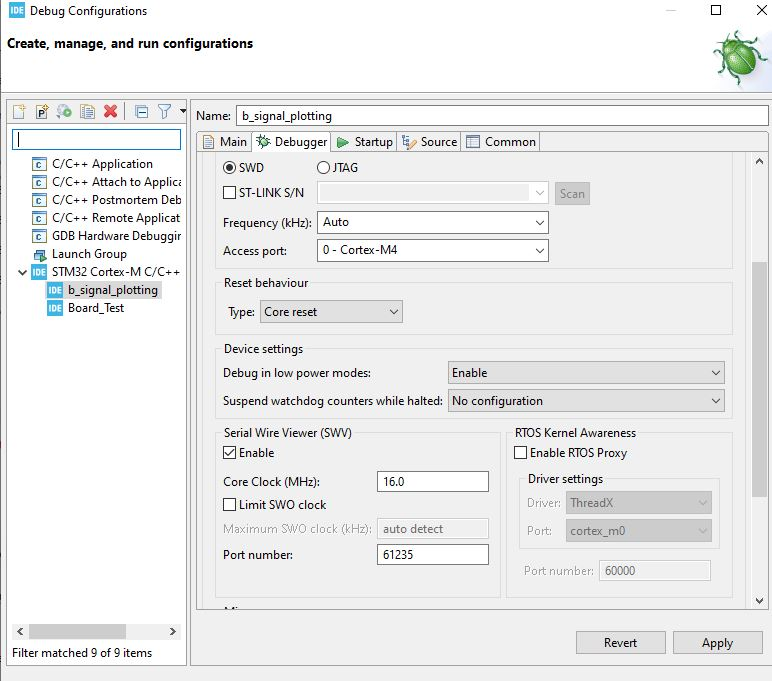
\includegraphics[scale=0.5]{Figures_DSP/chap_2_basics/debug_conf_swv_enable}
\caption{Enabling port to see global variable}
\label{fig:chap2_basics:debug_conf}
\end{figure}


    \item  When the window open, go to \verb|Debugger| tab, and enable \verb|SWV| option (stretch the window down if you don't see it)

    \item \verb|Window --> Show View --> SWV --> SWV Data trace timeline graph|


\item Now on the gear port, enable the global variable as shown in \autoref{fig:chap2_basics:enabling_port}


\begin{figure}[h]
\centering
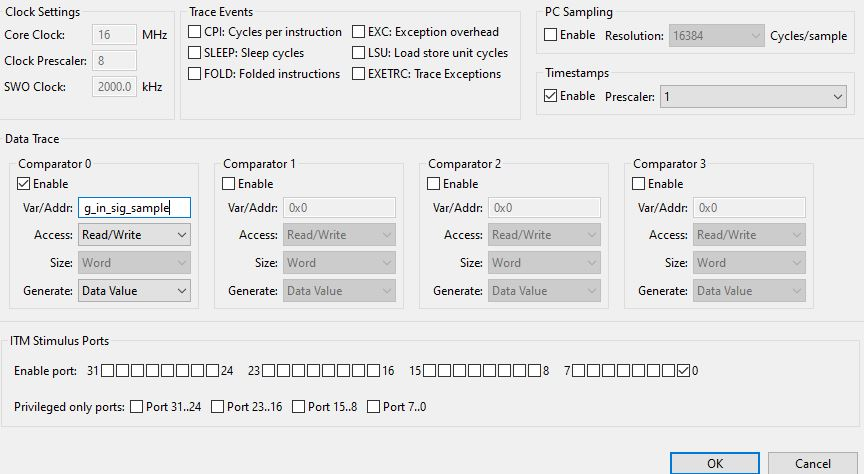
\includegraphics[scale=0.5]{Figures_DSP/chap_2_basics/enabling_port_see_global_var.JPG}
\caption{Enabling port to see global variable}
\label{fig:chap2_basics:enabling_port}
\end{figure}
      
\end{itemize}

\newpage

\section{Developing UART driver}

Now we will plot signal using UART protocol communication.

\subsection{Explanation of UART in stm32F411 nucleo}
\label{sub:Explanation of UART}

Important points:

\begin{itemize}

 \item When we open the data sheet to the function block diagram (page 15), we can see that we have many UART modules (\verb|USART1|,\verb|USART2|,$\cdots$).

\item We can see that at some \verb|USART2| for example, we have \verb|RX,TX| as \verb|AF| (in alternate function mode)

    \begin{itemize}
        \item Whenever we need to connect to some peripheral, we need to configure \verb|GPIO| pin (here in \verb|AF| mode to configure \verb|RX,TX|)
        
    \end{itemize}

\item  Because \verb|UART| is a physical communication protocol, it needs some wire to communicate. Now our computer doesn't have wires, but it has \verb|USB| port to communicate

    \begin{itemize}
        \item Now internally, \verb|USART2| is connected to the \verb|USB| port used to flash in and debug our microcontroller, so we can use it.

        \item  This is only true for nucleo board, discovery board for example doesn't have such connection in \verb|USART2|
    \end{itemize}


\item  Now \verb|TX,RX| are \verb|GPIO| in \verb|AF| mode, so we need to go to \verb|AF| mapping table, which can be found in the data sheet (Table 9 page 47)

    \begin{itemize}
        \item We can see by inspecting the table, that for \verb|USART2|, \verb|PA2| and \verb|PA3| are the port to be configured

        \item  Also we need to get need to configure clock configuration for \verb|PA|
    \end{itemize}

\item  Also, we can see from the functional block diagram that \verb|USART2| is connected to the \verb|APB1| bus, so we need to configure the clock of this bus 

\end{itemize}

\
\subsection{Developing Tx function}

In this section we develop the tx function.

Before writing the steps, let's summarize some important points from \ref{sub:Explanation of UART}

\begin{itemize}
    \item functional block diagram of stm32F411 nucleo board is on the data sheet document, page 15

        \begin{itemize}
            \item from this document we can see \verb|USART| peripheral, and we are going to use \verb|USART2|
        \end{itemize}

    \item  \verb|USART2| contains 2 pins \verb|RX| and \verb|TX| which are only some \verb|GPIO| pins in \verb|AF| mode (alternate function mode)

        \begin{itemize}
            \item To know the mapping of \verb|RX| and \verb|TX| to which \verb|GPIO| pins, we look at the \verb|AF| mapping table, found in the data sheet (Table 9 page 47): \verb|TX| $\mapsto$ \verb|PA2| and \verb|RX| $\mapsto$ \verb|PA3|
        \end{itemize}
    
\end{itemize}


Now let's do the development part.

\begin{itemize}
    \item configure \verb|GPIOA| clock: via \verb|RCC AHB1 ENR| register (because GPIOA uses \verb|AHB1| bus)
\end{itemize}


\newpage

\section{Summary Basic of Signals in stm32cube IDE}

\begin{itemize}
    
\item Peripheral types: core and manufacture \\

every microcontroller comes with 2 type of peripheral: a manufacturer peripheral (like USB,I2C,$\cdots$), and core peripheral (which are implemented by arm in our case). The FPU is one of these core peripheral, and to enable it, we nee to refer to \tbi{arm Cortex M4 generic user guide}





\end{itemize}










\end{document}



